\subsubsection{Архитектура Системы}

Учитывая опыт существующих разработок, направленных на решение поставленной задачи, а особенности {\it VBA} и {\it VSTA}, Была разработана концептуальная модель взаимодействия основных компонентов платформы.

\paragraph{Пару слов о выбранных технологиях}

В качестве внешней IDE для разработки расширений была выбрана IDE с открытым исходным кодом SharpDevelop. Этот выбор был сделан по нескольким причинам:

Во-первых, эта IDE может управляться программно извне при помощи встроенной технологии SDA. Программное управление позволяет выполнять различные действия в IDE без участия пользователя. Например, показывать или скрывать само приложение, запускать сборку проекта, управлять сохранением и загрузкой проектов, и многие другие. 

Во-вторых, эта IDE поддерживает плагины. Это свойство позволит добавить какую-либо отсутствующую в базовой поставке функциональность не меняя исходного кода самого SharpDevelop. Это важно, так как изменение исходного кода сделает неудобным распространение готовой платформы, так как она будет совместима только с конкретной сборкой SharpDevelop. Использование плагинов позволит добавить нужную функцинальность в уже установленный экземпляр этой IDE.

В-третьих, SharpDevelop поддерживает кастомизацию, то есть изменение своего внешного вида и поведения при момощи конфигурационных файлов. Под изменением внешнего вида нужно понимать удаление <<лишних>> в контексте данного сценария использования (как внешней IDE для разработки расширений) элементов управления, добавление новых элементов управления, управление доступностью этих элементов, и прочее. Изменение поведения состоит в подмене штатных обработчиков событий элементов управления (например, кнопок), на свои собственные обработчики с измененной логикой. Например, запуск отладчика не должен пытаться стартовать сборку самого расширения (это попросту невозможно, так как расширения представляет из себя библиотеку классов), а присоединить отладчик к процессу хост-приложения.

В-четвертых, открытый исходных код поможет быстрее решить проблемы, связанные с интеграцией SharpDevelop в разрабатываемую платформу, так как сама IDE может быть запущена под отладчиком.

\TODO{больше букв!!!! Еще больше!!!}

\begin{figure}[!h]
    \centering
    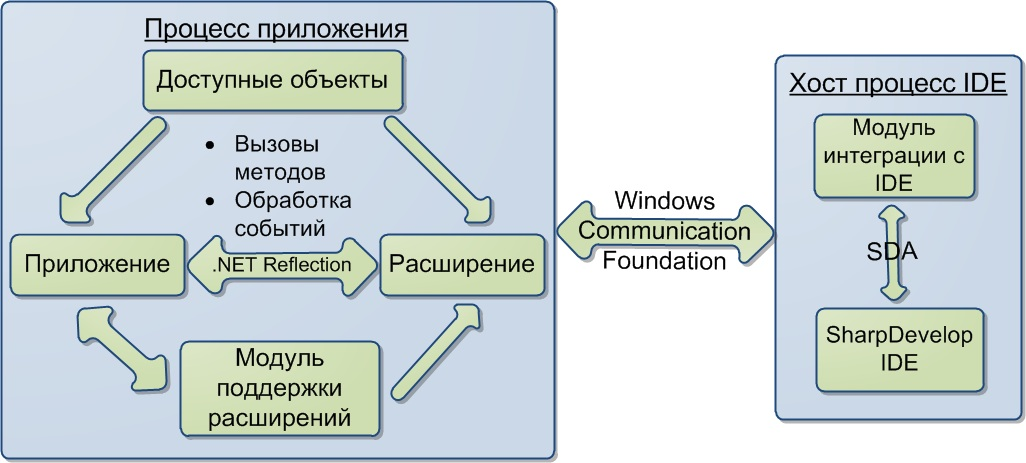
\includegraphics[width=15cm]{fw_arch1.jpg}
    \caption{Взаимодействие компонентов системы}
    \label{fw_arch1}
\end{figure}
